\documentclass{article}
\usepackage[utf8]{inputenc}
\usepackage{tikz, pgfplots}
\usepackage[T1]{fontenc}
\usetikzlibrary{positioning, automata}

\title{Graphs and Automata}
\begin{document}
\tableofcontents
\begin{center}
\maketitle

% Basic graph of discrete math
\section*{Basic Graph}
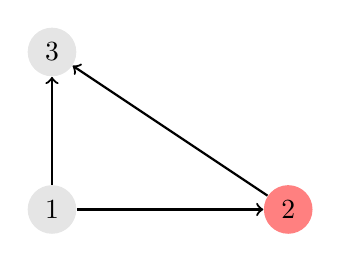
\begin{tikzpicture}
    % Styles
    \tikzstyle{vertex} = [circle, fill=black!10]
    \tikzstyle{selected vertex} = [vertex, fill=red!50]
    \tikzstyle{edge} = [->, thick]

    % Nodes
    \node[vertex] (v1) at (0, 0) {1};
    \node[selected vertex] (v2) at (3, 0) {2};
    \node[vertex] (v3) at (0, 2) {3};

    % Edges
    \draw[edge] (v1) -- (v2);
    \draw[edge] (v1) -- (v3);
    \draw[edge] (v2) -- (v3);
\end{tikzpicture}

\vspace{20pt}

% Automaton Example 1
\section*{Automaton Example 1}
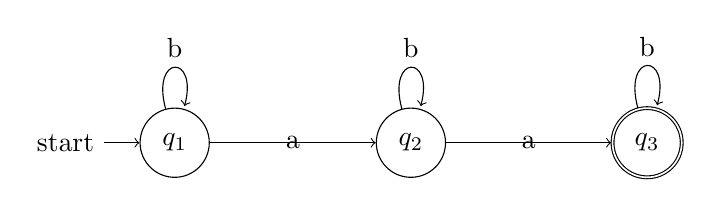
\begin{tikzpicture}[->, node distance = 3cm]
    % States
    \node[initial, state] (A) {$q_1$};
    \node[state] (B) [right of=A] {$q_2$};
    \node[state, accepting] (C) [right of=B] {$q_3$};

    % Transitions
    \path (A) edge[loop above] node {b} (A)
              edge node {a} (B)
          (B) edge[loop above] node {b} (B)
              edge node {a} (C)
          (C) edge[loop above] node {b} (C);
\end{tikzpicture}

\vspace{50pt}

% Automaton Example 2
\section*{Automaton Example 2}
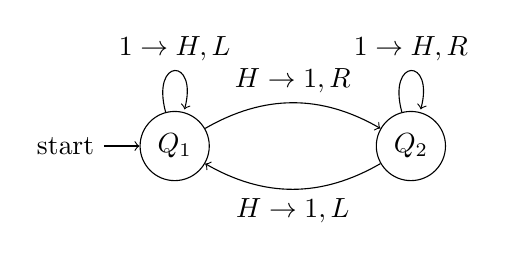
\begin{tikzpicture}[->, node distance = 3cm, auto]
    % States
    \node[initial, state] (A) {$Q_1$};
    \node[state] (B) [right of=A] {$Q_2$};

    % Transitions
    \path (A) edge[loop above] node {$1 \rightarrow H,L$} (A)
              edge[bend left] node {$H \rightarrow 1,R$} (B)
          (B) edge[bend left] node {$H \rightarrow 1,L$} (A)
              edge[loop above] node {$1 \rightarrow H,R$} (B);
\end{tikzpicture}

\vspace{50pt}

% Complex Automaton
\section*{Complex Automaton}
\begin{tikzpicture}[->, node distance = 3cm, auto]
    % States
    \node[initial, state] (A) {};
    \node[state] (B) [right of=A] {};
    \node[state] (C) [below of=A] {};
    \node[state] (D) [below of=B] {};
    \node[state] (E) [right of=D] {};

    % Transitions
    \path (A) edge[bend left] (B)
              edge (B)
          (B) edge[bend left] (A)
              edge (D)
          (C) edge (A)
              edge[loop below] (C)
          (D) edge (C)
              edge (E);
\end{tikzpicture}

\end{center}

\end{document}
